\documentclass[free]{flammie}

\usepackage{graphicx}

\title{Divvunspell---Finite-State Spell-Checking and Correction on Modern Platforms}

\author{Flammie A Pirinen \\
  Divvun \\
  UiT---Norgga árktalaš universitehta \\
  Tromsø, Norway \\
  {\tt flammie.pirinen@uit.no} \\\and%
  Sjur Nørstebø Moshagen \\
  Divvun \\
  UiT---Norgga árktalaš universitehta \\
  Tromsø, Norway \\
  {\tt sjur.n.moshagen@uit.no}}

\date{}

\begin{document}
\maketitle
\begin{abstract}
    Spell-checking and correction is one of the key applications of natural
    language support.  Historically, for the biggest, less morphologically
    complex languages, spell-checking and correction could be implemented by
    relatively simple means; however, for morphologically complex and
    low-resource languages, the solutions were often suboptimal.  Finite-state
    methods are the state of the art in rule-based natural language processing
    and also for spell-checking and correction they have been effectively used.
    In this article, we show some recent developments of a finite-state
    spell-checker implementation that works with modern operating systems and
    platforms.
\end{abstract}



\section{Introduction}

Spell-checking and correction is one of the most basic and most important
applications of natural language processing for standardised, written languages.
A spell-checker works as a tool for all of the writers of the language, ensuring
that most of the texts written follow a norm that is enforced by the tool.  This
has enormous significance for the text production in the language, which in turn
is becoming more and more important in the era of large language models.  A
large language model is built on huge quantities of texts written by humans, and
an underlying expectation is that the majority of the text is written in a
standard, norm-abiding language form.

Traditionally spell-checkers have been readily available for morphologically
simple languages but have had more limited success for more morphologically
complex languages; for example, to this day hunspell is popularly used for a lot
of platforms on a computer as a default spell-checker engine. Hunspell itself
being developed because previous systems were insufficient for Hungarian
morphology, it moreover is limited for other morphologically complex languages.
Another approach to spell-checking that is popular in contemporary systems is
data-based, either statistical or neural network, this is what many of the
autocorrect and autocomplete style models are based on.  This, on the other
hand, limits the low-resourced languages out of the equation.

The main contribution of this article is recent developments in our
implementation of \textit{finite-state spell-checking}, as well as relevant
tooling and automation.  Finite-state spell-checking works for morphologically
complex languages and does not necessarily require any training data, making it
suitable for low-resource use cases.  One emphasis of this article is the
developments related to full end-user use case of the method that the software
is not merely an academic experiment but a product that can be installed and
used by the language users.  For this purpose, we have developed automated
evaluation methodology as well as systems for automatically distributing the new
changes to end-users.

Following the recent trends of the language technology, that is the
break-throughs of the large language models and neural networks, we evaluate our
system and compare it to an out of the box neural network in a basic
spell-checking and correction task. While the evaluation we perform here is
quite rudimentary as a neural network application, it builds towards the
research question of: how and to which extents and in which parts of a
spell-checking and correcting system shall the large language models be used in
hybrid with existing finite-state and rule-based solutions.

\section{Background}

Spell-checking and correction is an application of natural language processing
that has been studied since the 1950's.  The earliest models worked in practice
based on static lists of correctly written word-forms to check against, then
slowly adding support for morphological processes as larger vocabularies and
more morphologically complex languages were implemented.  The most widely spread
versions of the spell-checkers used in personal computers are commonly known as
\texttt{*spell} software, from original SPELL to ispell, aspell, myspell,
hunspell and nuspell.  Still, these have been difficult to adapt for
morphologically rich languages, so for specific languages softwares like
zemberek for Turkish and hspell for Hebrew have been developed

Parallel to dictionary-based spell-checkers there has been statistical
approaches to spell-checking.  This is based on learning a language model from
large correctly written texts, one of the most influential models here
is~\cite{norvig2010howto}.  This line of models is usually a basis in most of
the mobile auto-complete and autocorrect style systems, nowadays likely based on
generative neural network models.

The most basic tool for modeling errors is based on the invention of edit
distance, where the errors are modeled as a combination of missing a letter,
adding an extra letter, using a wrong letter, or swapping two adjacent letters,
first introduced by~\cite{levenshtein1966binary}.  Other common ideas that have
been used include listing common confusables altogether, trying to map phonemic
errors to the writing system various ways, and weighing the mistakes made on a
keyboard by the keyboard layout.

One of the most popular ways of handling word-forms of morphologically complex
languages is Finite State Morphology~\cite{beesley2003finite}, this is often
considered the state of the art in handling rule-based language modeling of
morphologically context low-resourced languages to this date.  The finite-state
formulation of spell checking with statistically trained language and error
models has been researched by~\cite{pirinen2014state}.  This type of models is
also used by the spell-checking and correction solution we are presenting in
this article.



\section{Methods}

Finite-state spell-checking is based on using finite-state automata to model
both the correctly spelled words (language model) and mapping of the
misspellings from incorrect forms to correct word-forms.  In finite-state format
this means that there is an automaton that accepts the correctly spelled
word-forms and does not accept incorrectly spelled word-forms, and another
two-tape automaton that can relate incorrectly spelled word-forms to correctly
spelled word-forms.  The automata can be weighted and thus give an ordering to
correction suggestions as well as likelihoods for the words of the languages in
general.  This model has been introduced by at least~\cite{pirinen2010finite},
and the software introduced here is based on the same finite-state formulation.
For language models we have used freely available open source finite-state
models from the GiellaLT infrastructure~\cite{pirinen2023giellalt}.

The \textit{divvunspell}\footnote{\url{https://github.com/divvun/divvunspell}}
software we introduce in this article is implemented in the Rust programming
language and has bindings and implementations for modern operating systems and
mobile platforms: macOS systemwide, Windows systemwide and in MS Office,
LibreOffice on all desktop systems, and in iOS and Android keyboard apps. There
is also a REST API for web-based
clients\footnote{\url{https://api-giellalt.uit.no/speller/XX}, where XX is the
ISO 639 language code.}.  We have implemented some basic improvements to the
engineering and efficiency as well as correctness of the software.  The
published version is both light-weight and fast enough to be used as an
interactive spelling checker on average end-users' mobile platforms.  We have
fine-tuned the error-correction algorithm with adjustable weights in the errors
made in word-initial, word-medial and word-final positions separately; in the
the current version a spelling error in the first or last letter of the word
adds triple the weight of an error in the mid-word unless configured
otherwise.\footnote{the actual and up-to-date implementation of the algorithm
can be found on GitHub.} We have also developed an automated evaluation software
for the spell-checking software that can ensure the quality of the
spell-checking models does not degrade, as well as a continuous integration and
deployment system that can distribute the models to the end users when the
dictionaries or grammars of language models are updated, as long as the quality
of the spell-checker has not deteriorated.  The automatic evaluation tools are
available on the github repo of \textit{divvunspell} and their integration to
language development infrastructures can be found on the actual language data
repositories\footnote{\url{https://github.com/giellalt/template-language-und},
to be refactored into \url{https://github.com/divvun/actions/}}.

We experiment with a popular out-of-the-box large language model that is
available for most users free of charge via a chat interface.~\footnote{At the
time of writing we had access to a version of ChatGPT-4o.} We do not perform any
in-context learning or retrieval augmented generation, this is an initial
experiment towards potential hybrid models of finite state and neural models of
spell-checking and correction.

\begin{figure*}
    \centering
    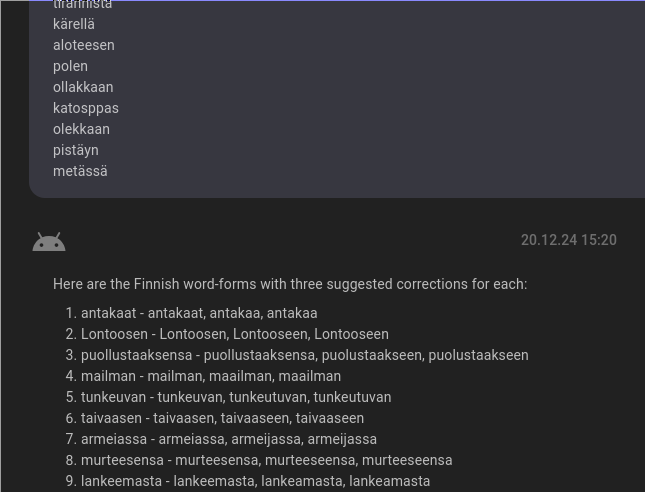
\includegraphics[width=.9\textwidth]{2024-12-20-152333_645x492_scrot.png}
    \caption{Example of LLM-based spell-checking and correction}\label{fig:overleaflink}
\end{figure*}


\section{Results}

We performed a small experiment to verify the working of our system and to see
how well the out-of-the-box neural network works on this task.  We are testing
with a real-world error corpus of Finnish word-forms---50 correctly written
words and 50 spelling mistakes found in a large corpus---by picking up
non-words and correcting them manually.  Finnish is a morphologically complex
language with medium-to-high resources.  The results are in
Table~\ref{tab:my_lael}.  The overall quality of both spelling checking and
correction is lower in the LLM-based system than it is for the rule-based system
but it still manages to provide correct suggestions almost as often as
rule-based system does.

\begin{table}[htb]
    \centering
    \begin{tabular}{crrr}
       System  &  1st & Any \\
       FST & 70~\% & 88~\% \\
       LLM & 50~\% & 85~\% \\
       % Anonymised  & 72~\% & 84~\% \\ % results for sme unverified
       % LLM & 44~\% & 49~\% \\ % results for sme unverified
    \end{tabular}
    \caption{Automatic evaluation of spelling correction }\label{tab:my_lael}
\end{table}

\section{Discussion and Future Work}

We have shown a software that brings the spell-checker to end-users on mobile
and desktop platforms and updates automatically when linguistic data gets
developed. However, especially on mobile platforms but also increasingly on
desktop, the spell-checking has been shifting towards a sub-function of a text
prediction subsystem, e.g. autocomplete / autocorrect. It would be interesting
future work to study possibility of such a system for morphologically complex
and low-resource languages.

We only performed cursory experiments to ensure that our system works within
specified parametres, the system should be functionally similar as the system
evaluated by~\cite{pirinen2014state} in their larger survey. We also performed
the same experiment on an out-of-the-box, not fine-tuned and not prompted,
re-inforced or otherwise context augmented neural network, mainly to find out
their current level of quality and possible future modes of hybridisation. From
the results it seems that the LLM-based systems are approaching the quality of
rule-based system in terms of overall suggestions but if you concentrate on
suggestion quality, it is still not comparable. More importantly, when doing a
manual error evaluation, we find some examples where rule-based system is more
restricted towards edit distance type error modeling, whereas LLM tends to
suggest patterns of related word-forms of a same word.

One of the requirements of an end-user system in spell-checking and correction
is high precision in detecting errors, the end-users tend to react very
negatively of spell-checking systems that red-underline words they know are
correctly written. Secondly the suggestions need to be reasonable first and
foremost. Both of these aspects are relatively harder to get right with LLM
solutions of today, however, there are some indications that LLMs can be more
creative in error modelling, and especially when the spelling-correctors are set
in the automatic text prediction context, they have been succesful. Ideally we
could foresee a future system that combines the high precision of rule-based
spell-checking with creative prediction of an generative AI as a potential
spell-checking system.


\section{Summary}

We have demonstrated a spell-checking and correction system based on
finite-state technology that works on end-user systems including desktop office
applications and mobile phones.  We tested an LLM-based approach to the same
task to see where they stand at and if they could be included in the system but
at the moment they are still far enough from end-user quality to be included
as-is.

\section*{Limitations}

The LLM test is based on one version of a closed commercial system and is not
reproducible. The test is only intended to give an impression of initial
usability of such systems, and for that reason we also have not included
extensive descriptions of the parameters, prompts and version specifics.  The
prompt used is given in the Figure~\ref{fig:prompt}.

\begin{figure}
\scriptsize
    \begin{verbatim}
You are a spell-checker for Finnish language,
you will be given a list of word-forms and you
should answer with a list of the word-forms,
then suggested corrections for example:
    rahhaa	rahaa	rahkaa
If a word is already correct,
the first suggestion should be
the same as the input word:
    päälle	päälle
    \end{verbatim}
    \caption{ChatGPT prompt for spell-checking.\label{fig:prompt}}
\end{figure}

\section*{Ethics Statement}

The data annotation and human evaluation was performed by article authors and
colleagues; no unpaid annotators were used.  The LLMs use significant amount of
water and electricity and we have made an effort to minimise unnecessary overuse
of LLMs.

% \section*{Acknowledgments}







\bibliographystyle{unsrt}
\bibliography{cgmta2025}

\end{document}
